\appendix
\setcounter{figure}{0}
\renewcommand{\thefigure}{A\arabic{figure}}
\renewcommand{\theHfigure}{A.\arabic{figure}}
\renewcommand{\theHequation}{A.\arabic{equation}}
\section{Viewing Geometry and Short-Arc Checks}
\label{app:checks}

\subsection{Solar elongation and angular rate}
\label{app:geometry}

Solar elongation is evaluated using target and
solar directions with a common observing
origin. The archived ALEPH calculation
subtracts the observer's heliocentric
position from the light-time-corrected
heliocentric asteroid position in
J2000-equatorial axes. In that same
representation, let $\boldsymbol{r}_{\rm o}$
be the observer vector and
$\boldsymbol{r}_{\rm a}(t-\tau)$ the
retarded asteroid vector. The unit
directions and elongation are
\begin{align}
\hat{\boldsymbol{u}}_{\rm a} &=
\frac{\boldsymbol{r}_{\rm a}(t-\tau)-\boldsymbol{r}_{\rm o}(t)}
 {|\boldsymbol{r}_{\rm a}(t-\tau)-\boldsymbol{r}_{\rm o}(t)|},\\
\hat{\boldsymbol{u}}_\odot &=
-\frac{\boldsymbol{r}_{\rm o}(t)}{|\boldsymbol{r}_{\rm o}(t)|},\\
\epsilon &= \cos^{-1}
  \left(\hat{\boldsymbol{u}}_{\rm a}\cdot
        \hat{\boldsymbol{u}}_\odot\right).
\end{align}
An independent calculation from the
archived DE432s Sun, Earth, and site
vectors agrees within $0.009\asec$
over the frozen matched epochs.

For the 531,612 primary associations
in validated exposures, the median
elongation is $149.34^\circ$. The
minimum, $59.72^\circ$, occurs for
(1520)~Imatra at 2026 January~26
10:35:38.531~UTC. At that epoch the
geometric solar and target altitudes
are approximately $-14.45^\circ$
and $+43.88^\circ$, respectively.
The elongation distribution in
Figure~\ref{fig:geometry} is weighted
by individual associations.

Angular rates instead use adjacent
pairs of associations belonging
to the same identity and physical
observing night, with different
exposures and a positive time
interval. We divide the great-circle
separation by that interval,
calculating rates separately from
predicted and measured positions.
There are 304,909 valid pairs,
with median predicted and measured
rates of 26.84 and
26.84~\rateunit\ after rounding.
The five pairs above
1,000~\rateunit\ belong to
2026~AA and 2026~CA and have
consistent predicted and observed
displacements. They are retained
as real fast-motion examples
within the known-association
sample.

\begin{figure}[tbp]
\centering
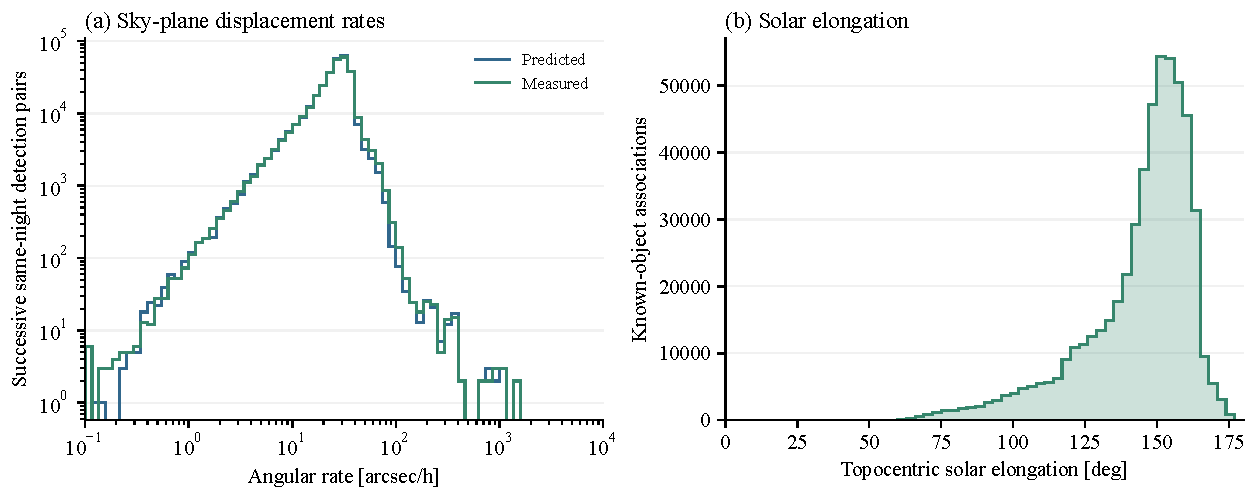
\includegraphics[width=\linewidth]{figA1_motion_and_solar_elongation.pdf}
\caption{Viewing geometry and angular
motion. The rate distributions use
304,909 adjacent within-night pairs
of distinct exposures for the same
known identity; predicted and
measured rates are calculated
separately from great-circle
separations. The elongation
distribution uses the 531,612
validated primary associations,
counting every association and
using the same observing origin
for the Sun and target.
The known-object sample is
not restricted to the
$3$--$63$~\rateunit\ interval
used by the independent
motion search.}
\label{fig:geometry}
\end{figure}

\subsection{Candidate timing and fit diagnostics}
\label{app:shortarc}

The historical short-arc calculation uses
equal endpoint heliocentric-distance
hypotheses with zero assumed radial
derivatives to construct the endpoints;
it does not continuously optimize
the two line-of-sight ranges.
The provisional tracklet-subset
search permits seeds with final-epoch
heliocentric speeds below
140~km~s$^{-1}$. The subsequent
refit returns to the
35~km~s$^{-1}$ acceptance limit
specified in
Section~\ref{sec:motion_method}.

Figure~\ref{fig:shortarc} compares
the exposure-midpoint span and
short-arc fit RMS of the 58
retained historical linkages.
The six links consistent with
C/2025~Y1 are marked separately.
The RMS summarizes internal
agreement over the observed
short arc; a small value with
only a few measurements does
not establish a unique
heliocentric orbit.

The original tracklet, link,
and orbit calculations used
exposure midpoints. The
historical unknown-candidate
ADES export instead wrote
exposure-start times. The
paper's 179-measurement table
uses the original exposure
duration to correct each
exported epoch to its
midpoint. The median offset
is $+15.0015$~s, corresponding
to a median along-track
displacement of $0.0617\asec$
and a maximum of
$0.2556\asec$ at the
measured rates. This
correction concerns the
reported measurement times;
it does not alter the
epochs used to construct
the original linkages.

The historical short-arc
implementation adopted the
same longitude as the
known matcher but latitude
$40.394239^\circ$ and
height 868.221~m. A
128-night sensitivity
comparison between these
two site specifications
found no change in the
stored fit-success or
diagnostic-quality
classification. The
as-executed coordinates
and the comparison are
preserved with the
analysis products.

\begin{figure}[tbp]
\centering
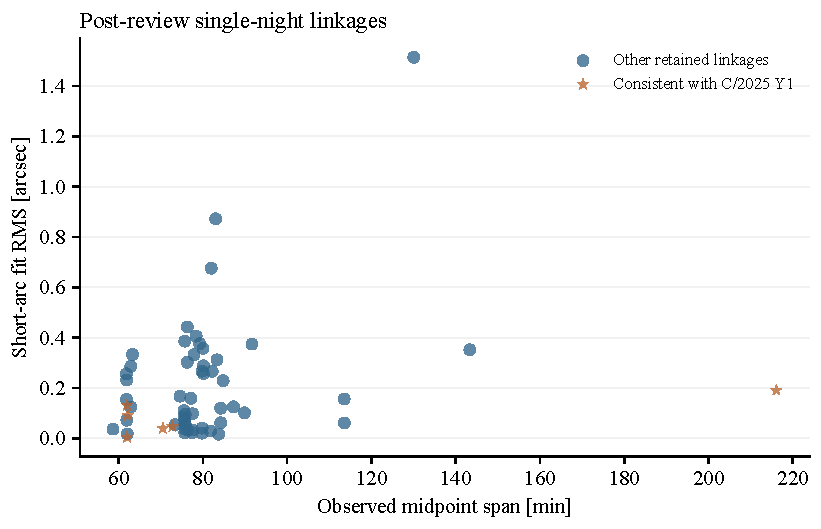
\includegraphics[width=0.75\linewidth]{figA2_candidate_short_arc_diagnostic.pdf}
\caption{Exposure-midpoint span and
short-arc fit RMS for the
58 image-reviewed historical
single-night linkages.
The six numerically
associated with C/2025~Y1
are shown separately.
These values describe
within-arc consistency,
rather than uncertainties
of uniquely determined
orbits.}
\label{fig:shortarc}
\end{figure}
